\documentclass[twoside, UTF8]{EPURapport}
%\usepackage{listings}

%\renewcommand{\lstlistlistingname}{Liste des codes}
%\renewcommand{\lstlistingname}{Code}

%\addextratables{%
%	\lstlistoflistings
%}

%\swapAuthorsAndSupervisors


\graphicspath{Image}

\thedocument{Type de document}{Le titre long}{Rapport de stage de fin d'étude}

\grade{Département Informatique\\ 5\ieme{} année\\ 2010 - 2011}

\authors{%
	\category{Étudiant}{%
		\name{Fan ZHAO} \mail{zhao.fan@etu.univ-tours.fr}
	}
	\details{DI5 2010 - 2011}
}

\supervisors{%
	\category{Encadrant}{%
		\name{François Benaiteau} \mail{francois@chugulu.com}
	}
	\details{Chugulu Games}
}

\abstracts{Description en français}
{Mots clés français}
{Description en anglais}
{Mots clés en anglais}

\begin{document}

\chapter{Introduction} % (fold)

Le stage en 5ème année, qui est le stage de fin des études, pour pouvoir obtenir le diplôme, est obligatoire pour tous les étudiants au département informatique. La durée est au minimum 4 mois, au plus 5 mois, soit 20 semaines, pendant l’été 2011. 

Le stage de fin des études est très important pour un étudiant. Parce que la durée de ce stage est 4 mois, qui sont plus longs qu'avant. Aussi, après ce stage, nous allons diplômer. Nous devons chercher un boulot et commencer travailler. Nous serons plus étudiants. La durée de 4 mois nous permet d'avoir de la chance de participer dans un Éque. Travailler au dessus dans un grand projet. Pour cette durée, notre mission n’est plus les petites. Cela nous permet de toucher des mécanismes d'une entreprise, des contrôles des projets, des nouvelles techniques, des applications au niveau d'entreprise, des façons au niveau d'entreprise pour développer, etc. Aussi, nous pouvons rencontrer les gens, apprendre les nouvelles idées, etc. De l'autre coté, ce stage nous permet de savoir ce que nous en avons besoins, ce que nous aimer. Il est important puisqu’il y aura de la chance pour nous de continuer travaillé après stage. Même si nous n'aurons pas de chance de continuer, il peut nous donner quelques idées pour nous aider dans la future de recherches des travaux. Nous sommes bénéficié aussi à partir de ce stage, est que nous pouvons observer une vraie entreprise. Cela peut nous aider pour créer notre propre entreprise dans la future.

J’ai eu de la chance de trouver un stage dans l’entreprise Chugulu Games, qui est une entreprise à Tours, spécialisée dans le secteur des jeux. Mon stage a commencé du 23 mai, jusqu'au 30 septembre. Je travaille comme un développeur iOS. Ce stage est important pour moi, puisque travailler comme un développeur iOS est mon rêve. 

% chapter Introduction (end)

\chapter{Présentation} % (fold)

\section{Présentation de l'entreprise} % (fold)

\subsection{Chugulu Games} % (fold)

Chugulu Games est un studio de création spécialiste de la communication ludo-interactive et de l'advertainment. C'est concevoir et fabriquer des créations digitales (advergames,gaming banners, quiz interactifs, jeux multi-joueurs, serions games, social média applications) dont la dimension ludo-interactive, virale et communautaire est un accélérateur de notoriété et d'image de marque.

Voici le logo~\ref{fig:Image_Chugulu_Games1} de Chugulu Games.

Créée en 2006, Chugulu Games est une société spécialisée en advertainment. Nous concevons et fabriquons des créations digitales dont les dimensions ludique, virale et communautaire sont des accélérateurs de préférence de marque, de notoriété et de traffic.

Chugulu Games se concentre principalement sur 4 domaines principalement : Social Games, Jeux iPhone, Online Games et Unity 3D games. Comme le Figure~\ref{fig:Image_Chugulu_Games1} 


\begin{figure}[htbp]
	\centering
		
\includegraphics[width=6in]{Image/Chugulu-Games1.jpg}
	\caption{Logo de chugulu}
	\label{fig:Image_Chugulu_Games1}
\end{figure}

Principalement dire, Chugulu games a 2 type de jeux suivant le techniques utilisés. Un type est le jeu sur internet, souvent développé par flash. Ce type de jeu contient le jeu <BlindTest> qui a un site web de chugulu, souvent, les autres jeux sont basés sur des sites web sociale. Par exemple, facebook. L'autre type principal est le jeu sur iPhone. Chugulu games commence a développer des jeux de 3D basé sur Unity 3d. 

% subsubsection Chugulu Games (end)

\subsection{Equipe} % (fold)
\label{sub:subsection_name}

Chgulu games a 2 équipes. Une équipe est à paris, qui sont l'équipe principale, l'autre équipe est aux état-unis. Les 2 équipes sont présenté par le Figure~\ref{fig:Image_EquipeChugulu} suivant:

\begin{figure}[htbp]
	\centering
		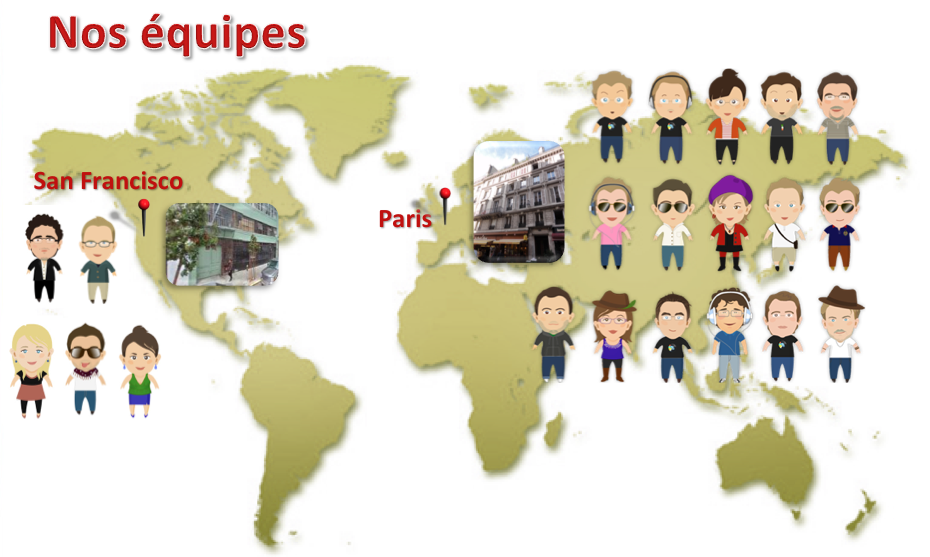
\includegraphics[width=6in]{Image/EquipeChugulu.png}
	\caption{L'équipe de chugulu games}
	\label{fig:Image_EquipeChugulu}
\end{figure}

Principalement dire, Chugulu games a 2 types de jeux suivant le technique utilisé. Un type est le jeu sur internet, souvent développé par flash. Ce type de jeu contient le jeu <BlindTest> qui a un site web de chugulu, souvent, les autres jeux sont basés sur des sites web sociaux. Par exemple, facebook. L'autre type principale est le jeux sur iPhone. Chugulu games commence a développer des jeux de 3D basé sur Unity 3d. 

% subsubsection Chugulu Games (end)


\subsection{Localisation} % (fold) \label{ssub:subsubsection_name}

Les jeux de chugulu games tous ont multi-language. Normalement, les jeux de chugulu games ont des versions d'anglais, version de français, version d'éspagnol. 

% subsubsection subsubsection_name (end)

\subsection{Références} % (fold) \label{ssub:références}

Chugulu games a travaillé avec plusieurs entreprises. Ses partenaires comportent des plus grandes entreprises françaises. Chugulu games a créé des jeux d'avertissements soie sur facebook, soie sur iPhone. Voici une liste des jeux.

Le Figure~\ref{fig:Image_chugulu_reference} liste quelques partenaires : 

% TODO chugulu references.


\begin{figure}[htbp]
	\centering
		
\includegraphics[width=6in]{Image/chugulu_reference.png}
	\caption{Les référence des produits de chugulu games}
	\label{fig:Image_chugulu_reference}
\end{figure}


\begin{itemize}
	\item LCL Open crémaillère \& 6:AM: Aménager entièrement son appart virtuel, et gagner réellement un an de loyer 
	\item Nokia Golden Goal \& Wunderman : Un advergame permettant de marquer plus de buts que l'équipe de France!
	\item Orange Snowballs \& Publicis Net : Un advergame pour i-Phone recréant une bataille de boules de neiges
	\item Air France \& La Chose : Un advergame s'inspirant du planisphère du magazine Air France
	\item Axe \& Buzzman : Un advergame prolongeant le film viral <<Canadairman>> pour la sortie d'AxeDry
	\item SFR \& EURO RSCG BETC 4D : Une réadaptation du Snake nokia 
	\item Renault \& Publicis Net : Contrer l'invasion de la dernière Scenic par des lapins vraiment très crétins
	\item Voyages SNCF \& Artdicted : Une narration ludo-pédagogique sur les gestes responsables du voyageur
	\item Prisma Press Group : Starbank, la bourse des people 
\end{itemize}

% subsubsection références (end)

\section{Advergame} % (fold) \label{sub:advergame}

\subsection{Définitions} % (fold) \label{ssub:définitions}

\begin{description}  \item[Advergame] : jeu développé pour le compte d’un annonceur.

\item[Casual gaming (ou jeu grand public)] : se dit des jeux vidéo s'adressant au plus grand nombre, femmes et seniors compris. Jeux présentant des gameplays simples et efficaces, compréhensibles en quelques secondes. Ex: PacMan, Tetris, AngryBirds, Doodle Jump, etc.

\item[Social gaming] : jeux grand public (ou pas) conçus pour être distribués sur les réseaux sociaux (facebook en particulier) dont les gameplay inclus des fonctionnalités sociales et virales. Ex : Farmville, Diner Dash, Mafiawars, etc.

\item[Serious game] : expérience ludique reprenant les codes du jeu vidéo, en vue de transmettre des acquis pédagogiques, responsables et/ou professionnalisants.

\item[Freemium] : modèle dans lequel la découverte du jeu est gratuite (free) et le gameplay propose des biens virtuels payants (premium).
\end{description}
Le définition sur le site Wikipédia est : L'advergame ou jeu vidéo publicitaire est un jeu vidéo qui cherche uniquement à promouvoir l'image d'une marque. Le mot advergame est un néologisme peu utilisé en France qui vient de la contraction de advertising (publicité) et de game (jeu). Un jeu vidéo publicitaire n'est pas à proprement parlé un serions game (jeu sérieux). Les serions games sont en effet des applications utilisant les technologies, techniques et usages du jeu vidéo, mais dans un but non ludique: apprendre à faire la cuisine, apprendre à faire quelque chose (médecine, etc.), etc.
Le jeu vidéo publicitaire est un jeu à part entière avec son côté ludique et justement non sérieux. C'est ce qui attire les annonceurs: l'univers jeu vidéo.

\subsection{Le marché de l'advergaming} % (fold) \label{ssub:le_marché_de_l_advergame}

Advergaming est un grand marché. Chiffre d’affaires mondial de 300 millions d’euros en 2010. Un taux de croissance annuel estimé à 47\% sur 2010 - 2015. Chiffre d’affaires 2015 estimé à 2 milliards d’euros. 40\% du top 100 des annonceurs français ont déjà eu recours à l’advergaming.

Au niveau de Fidélisation accrue des consommateurs, 61\% des joueurs déclarent avoir une meilleure opinion des produits présentés par un advergame. 50\% de la génération Y considèrent une marque plus crédible lorsqu'elle communique par le jeu.

Au niveau de Conversion prospect/client augmentée, 45\% des internautes satisfaits d’un advergame deviennent client de la marque.

% subsubsection le_marché_de_l_advergame (end)

% subsubsection définitions (end)

% subsection advergame (end) \subsection{Expérience technique} % (fold) \label{ssub:expérience_technique}

Chugulu game utilise plusieur techniques pour les jeux selon les besoins. Principalement, il existe 4 types de techniques. Ces 4 techniques sont les techniques moderne et populaire. 

\begin{description}  \item[Ruby on Rails] Rails est un framework open-source optimisé pour le bonheur des développeurs, engendrant une productivité accrue. Il combine simplicité, efficacité et modularité, ce qui nous permet de répondre facilement et rapidement aux besoins de nos clients. Utilisé par un nombre croissant de sites internationaux majeurs (Twitter, Yellow Pages, Github, Justin.tv, etc.), Ruby on Rails fait partie à ce jour des technologies web les plus dynamiques et les plus intéressantes de par sa communauté.

\item[Flash] est de très loin la solution la plus populaire pour diffuser du contenu interactif sur le web, car il est présent, selon Adobe, sur 99,5\% des ordinateurs connectés à Internet en Europe. La popularité de son clayer fait d’Adobe Flash un outil de développement et d’animation 2D très utilisé pour les jeux sur le web et pour les applications internet riches.

\item[L'iPhone] est aujourd'hui et depuis plusieurs années l'une des plateformes mobiles la plus plébiscitées par les usagers. Récemment l'iPad n'a fait que renforcer cette réalitée, c'est donc tout naturellement que Chugulu a consolidé son expérience dans cette technologie et plus largement dans les technologies mobiles.

\item[Unity 3D] Particulièrement concerné par les technologies les plus innovantes, Chugulu s’est familiarisé avec Unity3D, un moteur de rendu 3D destinée au développement de jeu vidéo jouables directement en page web, mais aussi sur iPhone, iPad et les smartphones Android. Son moteur graphique << next gen >> permet de créer des jeux proposant des rendus exceptionnels, disponibles sur un maximum de plateforme.
\end{description} % subsubsection expérience_technique (end)

\section{Introduciton au stage} % (fold)
Le mission de mon stage de fin d'études est développement et suivi des applications iPhone de la société. L'objective contient ces quatre points suivants : 


Mon stage à Chugulu Games peut être divisé en 2 parties. La première partie a duré 1 mois, commencé au début du stage. La première partie de stage s'est signifiée à travailler sur un projet qui s'appelle <<Télé7Jeux>>. La deuxième partie de stage a duré 3 mois, qui est la mission principale de mon stage. Dans la deuxième partie, j'ai travaillé sur un projet qui s'appelle <<Playboy-Spots>>.
\begin{itemize}  \item Savoir travailler en équipe.


\item Etre autonome sur une mission.

\item Respecter les consignes du lead développer iPhone  \item Faire preuve d'initiatives.
\end{itemize}


Mon stage à Chugulu Games peut être divisé en 2 parties. La première partie a duré 1 mois, commencé au début du stage. La première partie de stage s'est signifié à travailler sur un projet qui s'appelle <<Télé7Jeux>>. La deuxième partie de stage a duré 3 mois, qui est la mission principale de mon stage. Dans la deuxième partie, j'ai travaillé sur un projet qui s'appelle <<Playboy-Spots>>.


\subsection{Introductions au projet <<Télé7Jeux>>} % (fold) \label{ssub:introductions_au_projet_télé7jeux}

\begin{figure}[htbp]
	\centering
		
\includegraphics[height=3in]{Image/tele_7_jeux_logo_lien_logo.jpg}
	\caption{Le logo de télé7jeux sur iOS}
	\label{fig:Image_tele_7_jeux_logo_lien_logo}
\end{figure}


<<Télé7Jeux>> est un projet sur iPad. Il est annoncé par l'entreprise <<Lagardere>>. Ce jeu comporte tous les télé7jeux sur iPad, y compris <<Jeu de mémoire>>, <<Mot de réfléchir>>, <<Mot de croix>>, etc.. Ce projet est de mettre tous les jeux de télé7 sur iPad.
J'ai travaillé dans ce au début du stage. Le jour quand j'étais à Chugulu game, la game désigne a été déjà fini. Ce que j'ai fait est essayer de sortir une version prototype du jeu <<Jeu de mémoire>>. Le principe de prototype est d'essayer de développer une version qui fonctionne, sans graphiques, et donner une impression aux games désignées pour qu'eux, ils puissent savoir le résultat de leur designer. 


En fait, <<Télé7Jeux>> est un gros projet. Le prototype fait par moi est un des 5 jeux, qui est le plus simple, qui s'appelle <<Jeu de mémoire>>. Comme un débutant de développeur d'iOS, c'était super bien pour moi d'appliquer ce que j'ai appris, de comprendre les règles, les conventions de Chugulu Games. J'ai pris beaucoup de temps pour se familier avec les conventions des nommages, les règles des entreprises, les styles des codes, les façons des communications, les processus de travailler ensemble avec les membres dans l'équipe, etc. 

Cette partie de stage, même si qui n'a que duré un mois est hyper important pour moi.

% subsubsection introductions_au_projet_télé7jeux (end)

\subsection{Introduction au projet <<Playboy-Spots>>} % (fold) \label{ssub:introduction_au_projet_playboy_s}


\begin{figure}[htbp]
	\centering
		
\includegraphics[height=3in]{Image/logoPlayboy.png}
	\caption{Logo de <<Playboy-Spots>>}
	\label{fig:Image_logoPlayboy}
\end{figure}




Ce jeu signifie à créer un jeu sur iPhone, qui est un jeu comme les autres jeux du type 'différence'. De plus, ce jeu ressemble beaucoup à un des 5 jeux dans <<Télé7Jeux>>. Donc, nous avons mis beaucoup de temps pour discuter si nous pouvons utiliser les même, et les partagé entre les 2 projets. Après examiner au niveau du code, au niveau des concepts, au niveau de l'outil de version contrôle. Il nous semble impossible d'atteindre ce but. En fait, le gros problème est que, même si les 2 jeux ont les mêmes conceptions, ils ont quand même beaucoup de différences dans la base, qui nous bloque.

Ce projet va sortir 2 versions totalement sur App Store - une boutique d'Apple qui permettre aux entreprises de publier et vendre leurs applications. Les 2 types est la version Lite - qui est en fait la version gratuit, et la version Prenium - qui est en fait la version payante. Les différences entre ces deux versions peuvent être résumé comme :  \begin{itemize}  \item La version lite contient un nombre de photos fixé. 

\item La version Prenium contient une boutique qui fournit le possibilité d'acheter plusieurs packs dans le jeu. 
\end{itemize}
Ce modèle de business est utilisé souvent par les entreprises des jeux. 

Sauf la boutique, ce jeu comporte la synchronisation de serveur qui sert à télécharger les images, reporter les scores, reporter les stats des joueurs, recevoir les notifications, etc.. Un score board local basé sur la base des données locale et un score <<Game Center>> basé sur Apple.

Ce projet a commencé un mois après le début de mon stage. J'ai travaillé comme un membre dans l'équipe mobile. Le mois au début de ce projet, j'étais le seul développeur qui travaille sur ce projet. Pendant cette durée, j'essayer de sortir la structure des jeux, choisi les techniques utilisés, développés la première version, qui est en fait le prototype du jeu. A partir de deuxième mois, tous les autres développeurs ont joint dans ce projet, nous commençons ce projet.


Ce projet est le premier projet que je travaille dessus au début jusqu'à la fin. Dans ce rapport, je vais parler de ce projet.

% subsubsection introduction_au_projet_playboy_s (end)


% subsection Introduciton au stage (end)
% chapter Présentation (end)




\chapter{Conclusion}

\annexes

\end{document}

